\documentclass[abstract=on,10pt,a4paper,bibliography=totocnumbered]{article}
\usepackage[paper=a4paper,left=35mm,right=35mm,top=25mm,bottom=30mm]{geometry}
\usepackage[doublespacing]{setspace}
\usepackage[english]{babel}
\usepackage[utf8]{inputenc}
\usepackage[round]{natbib}
\usepackage{amsmath}
\usepackage{colortbl}
\usepackage{amsfonts}
\usepackage{amssymb}
\usepackage{gensymb}
\usepackage{graphicx}
\usepackage{tikz}
\usepackage{enumerate}
\usepackage{enumitem}
\usepackage{subcaption}
\usepackage{booktabs}
\usepackage[hidelinks]{hyperref}
\usepackage[nameinlink]{cleveref}
% \usepackage{lineno}
\usepackage{multirow}
\usepackage{arydshln}
\usepackage[flushleft]{threeparttable}
\usepackage[nomarkers, nolists]{endfloat}
\usepackage[colorinlistoftodos]{todonotes}
\usepackage{scalerel}
\usepackage{tikz}
\usetikzlibrary{svg.path}

%------------------------------------------------------------------------------
%	Some Styling
%------------------------------------------------------------------------------
% Creating some TikZ styles
\tikzset{
  nonterminal/.style = {rectangle
    , minimum size = 6mm
    , very thick
    , draw = black!
  }
}

% Changing the style of captions in figures etc.
\captionsetup{labelfont=bf, format=plain, font=small}

% Change how equations are referenced
\renewcommand{\theequation}{Equation \arabic{equation}}%

% To be able to put an ORCID
\definecolor{orcidlogocol}{HTML}{A6CE39}
\tikzset{
  orcidlogo/.pic={
    \fill[orcidlogocol] svg{M256,128c0,70.7-57.3,128-128,128C57.3,256,0,198.7,0,128C0,57.3,57.3,0,128,0C198.7,0,256,57.3,256,128z};
    \fill[white] svg{M86.3,186.2H70.9V79.1h15.4v48.4V186.2z}
                 svg{M108.9,79.1h41.6c39.6,0,57,28.3,57,53.6c0,27.5-21.5,53.6-56.8,53.6h-41.8V79.1z M124.3,172.4h24.5c34.9,0,42.9-26.5,42.9-39.7c0-21.5-13.7-39.7-43.7-39.7h-23.7V172.4z}
                 svg{M88.7,56.8c0,5.5-4.5,10.1-10.1,10.1c-5.6,0-10.1-4.6-10.1-10.1c0-5.6,4.5-10.1,10.1-10.1C84.2,46.7,88.7,51.3,88.7,56.8z};
  }
}
\newcommand\orcid[1]{\href{https://orcid.org/#1}{\mbox{\scalerel*{

\begin{tikzpicture}[yscale=-1,transform shape]
  \pic{orcidlogo};
\end{tikzpicture}
}{|}}}}

%------------------------------------------------------------------------------
%	Titlepage: Header
%------------------------------------------------------------------------------
\title{Flooding of the Okavango Delta influences Connectivity for Dispersing
African Wild Dogs}

% List of Authors
\author{
  David D. Hofmann\textsuperscript{1,2,\S} \orcid{0000-0003-3477-4365} \and
  Gabriele Cozzi\textsuperscript{1,2} \orcid{0000-0002-1744-1940} \and
  John W. McNutt\textsuperscript{2} \and
  Arpat Ozgul\textsuperscript{1} \orcid{0000-0001-7477-2642} \and
  Dominik M. Behr\textsuperscript{1,2} \orcid{0000-0001-7378-8538}
}

% Reduce spacing between authors
\makeatletter
\def\and{%
  \end{tabular}%
  \hskip -0.5em \@plus.17fil\relax
  \begin{tabular}[t]{c}}
\makeatother

% Current Date
% \date{\today}

% And here the masterpiece begins
\begin{document}

% Change page numbering
\pagenumbering{gobble}

% Required to be able to cite
\bibliographystyle{apalike}

% Create Titlepage
\maketitle

%------------------------------------------------------------------------------
%	Titlepage: Additional Info
%------------------------------------------------------------------------------
\begin{flushleft}

\vspace{0.5cm}

\textsuperscript{1} Department of Evolutionary Biology and Environmental
Studies, University of Zurich, Winterthurerstarsse 190, 8057 Zurich,
Switzerland.

\textsuperscript{2} Botswana Predator Conservation Program, Private Bag 13,
Maun, Botswana.

\textsuperscript{\S} Corresponding author (david.hofmann2@uzh.ch)

\vspace{4cm}

\textbf{Running Title:} None

\vspace{0.5cm}

\textbf{Keywords:} Seasonal Flooding of the Okavango Delta and its Consequences
for African Wild Dog Connectivity

\end{flushleft}

%------------------------------------------------------------------------------
%	Abstract
%------------------------------------------------------------------------------
\newpage
\begin{abstract}
Climate change is expected to considerably impact vital rates of endangered
species. In particular dispersal, the phase during which species leave their
natal area and attempt to find a new territory to settle, may

We utilize seasonal changes in the flooding regime across the Okavango delta as
a large scale natural experiment to investigate how environmental changes impact
species' ability to disperse, and utlimately connectivity between remaining
subpopulations. Specifically, we apply individual-based dispersal simualtions to
simulate dispersal trajectories under two extreme scenarios, assuming minimal
and maximum flood extents.

Our results show that during years of minimum flood extent, the Okavango delta
releases vast areas that dispersers use as movement corridors, whereas during
years of extreme flood the delta's floodwaters pose a considerable dispersal
barrier that forces dispersing individuals closer towards human settlements.
Besides a better understanding of the conservation needs for the African wild
dog, our study also provides evidence that incorporating seasonality in studies
of connectivity is imperative to more accurately predict the dispersal ability
of endangered species.

\end{abstract}

%------------------------------------------------------------------------------
%	Main Text
%------------------------------------------------------------------------------
\newpage

\onehalfspacing
\tableofcontents
\doublespacing

% Change page numbering
\newpage
\pagenumbering{arabic}

% Create linenumbers
% \linenumbers

\section{Introduction}
\subsection{Climate Change}
\subsection{Vital Rates}
\subsection{Dispersal}
\subsection{Connectivity}
Dispersal is an important, if not the important, driver of landscape
connectivity and therefore of major interest to conservation authorities.

\subsection{Okavango Delta and African Wild Dogs}
The Okavango delta in Southern Africa poses a unique opportunity to study the
impacts of environmetal change on species dispersal ability and connectivity in
large scale natural experiment setup.


\section{Methods}
Programming language, packages, etc.

\subsection{Study Area}
The study area for this analysis was focused on the Okavango delta and its
surroundings in Southern Africa, comprising parts of Angola, Namibia, Botswana,
Zimbabwe, and Zambia \Cref{StudyArea}. To accomodate for the long distance
dispersal events commonly observed in the African wild dog, we considered a
large rectangular extent stretching from ... to ...., totalling to an area of xx
km. The dominant geographical feature in this region is the Okavango delta, the
world's largest inland delta and main driver of seasonal environmental change in
the region. While local rainfalls marginally impact water levels across the
delta, the main flood-pulsing rythm is driven by the water-influx from the
Okavango river. The Okavango carries rain waters collected the Angolian
highlands into the delta's distributaries. Although precipitation in Angola
peaks around ..., the water arrives in the delta with a delay of ... It only
slowly descends through the delta and reaches the distal ends (at the faults)
around ... At minimum extent, the flood covers an area of around xx km, whereas
during maximum flood it covers ... Vegetation in the study area can largely be
categorized into dense mopane forest, mixed acacia woodland, and plain
grassland. Human influence in the study area is generally low and mainly
concentrated to small villages at the western periphery of the delta, as well as
to the city of Maun at the southern tip of the delta. Large portions of land are
dedicated national parks, game reserves or forest reserves and the area is part
of the world's largest transboundary conservation initiative, the
Kavango-Zambezi Transfrontier Conservation Area.

\begin{figure}
  \begin{center}
  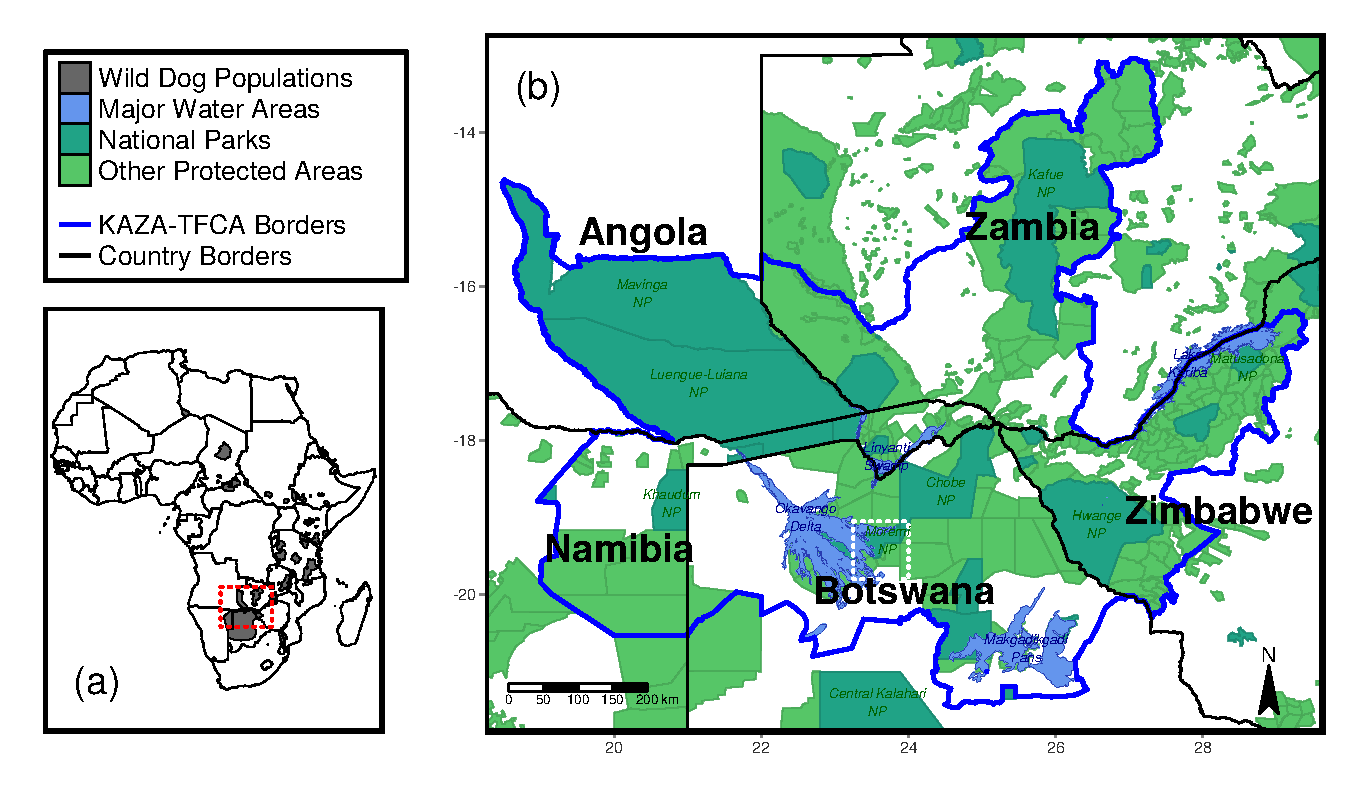
\includegraphics[width = \textwidth]{99_StudyArea.png}
  \caption{Study area across which we simulated dispersal events. Virtual
  dispersers were released at random locations within the orange source areas.}
  \label{StudyArea}
  \end{center}
\end{figure}

\subsection{Spatial Habitat Layers}
We represented the physical landscape through which dispersers could move by a
set of spatially referenced habitat layers each resolve at 250m x 250m. The set
of layers included water-cover, distance-to-water, tree-cover,
shrub/grassland-cover, and a human influence layer depicting anthropogenic
influences through villages, roads, and agriculture. A detailed description of
the different layers is provided in \Cref{Hofmann.2021}. Importantly, the
water-cover and the derived distance-to water layers were generated using MODIS
Terra satellite imagery, which enabled us to generate weekly updated layers that
provided detailed information about the flood-extent at any given point in time.
We had a total of 8xx remote sensed floodmaps at our disposal and used them to
generate two extreme scenarios; a minimal and maximum flood scenario. To create
the minimum flood scenario, we tallied the 50 floodmaps with smallest flood
extent into an average image. Finally, we created a binary map... Similarly, we
created an average image for high flood using the 50 most flooded maps. The
resulting maps are depicted in \Cref{FloodExtent}. For completeness we also
generated an  ``average'' floodmap by averaging across all 800 floodmaps
available to us. The results based upond this layer are presented in the
Appendix.

\begin{figure}
  \begin{center}
  \includegraphics[width = \textwidth]{99_FloodExtent.png}
  \caption{}
  \label{FloodExtent}
  \end{center}
\end{figure}

\subsection{Dispersal Model}
Our dispersal model was based on a previously parametrized and validated
\textit{integrated step-selection function (iSSF)} applied to the dispersal data
of 16 dispersing African wild dogs inhabiting the surroundings of the Moremi
National Park in the Okavango delta \citep{Hofmann.2021}. The iSSF model
consists of two complementary ``kernels'' plus their interactions. The first
kernel is a movement kernel and describes general movement behavior of
dispersing AWDs, irrespective of habitat conditions. The second kernel is a
habitat kernel and describes preferences of AWDs with regards to environmental
conditions. Finally, the model also includes interactions among the two kernels
and therefore allows to render how movement behavior changes depending on
habitat conditions.

\subsection{Source Areas}
We simulated dispersing AWDs originating from nine distinct source patches
located in the vicinity of the Okavango delta. The source areas were generated
as follows. First, we overlayed the OD with an oval that was bound by
geographical landmarks; in the north, the oval was bound by the Inflow of the
Okavango river into the ``pan-handle'' of the OD, north-east the oval was bound
by the Selinda-Spillway and the Linyanty swamp, towards South-East it was bound
by the Boteti river, and towards South-West by Lake Ngami. We then dissected the
polygon into five distinct patches using the same natural landmarks
(\Cref{StudyArea}). Patch one was given by the area south of the Boteti river
and area two by the area north of it up until the panhandle. Area three
stretched from the region easf of Maun towards north until the Selinda-spillway,
whereas area four stretched north of the spillway until west towards the
panhandle. Finally, a fifrth source area marked the peninsuale in the center of
the OD. In addition to these five source patches, we also distributed small
peripheral patches that we used to simulate individuals immigrating
\textit{into} system and to keep track of individuals leaving it.

\subsection{Dispersal Simulation}
For both environmental scenarios we simulated 1'000 individuals dispersing from
each of the nine source area depicted in \Cref{StudyArea}. The simulation
algorithm was based on the algorithm described in \Cref{Hofmann.2022} and works
as follows. A random location within the source area is chosen as a starting
point. Originating from the starting point, a set of 25 random steps are
generated by sampling step lengths from a gamma distribution fitted to observed
steps (what is a step?) (shape = , scale = ) and turning angles from a uniform
distibution on ($-\pi, +\pi$). Along each random step the underlying spatial
covariates are extracted and relevant movement metrics are computed (i.e.
log(sl), cos(ta), ta). The parametrized dispersal model is used to predict the
probability of each step for being chosen given the steps covariate values. One
of the steps is sampled based on assigned probabilities and the location of the
animal is updated. The procedure is then repated until the desired number of
steps (in our case 2000) is realized. Resulting trajectories resemble correlated
random walks. As the original model was trained using 4-hourly steps, a
simulated step also resembled straight line movements within four hours.

% We used a previously parametrized dispersal model to simulate dispersal
% trajectories of African wild dogs across the study area. To simulate dispersing
% wild dogs, we employed the simulation framework presented in
% \cite{Hofmann.2022}. In this framework, a movement model that renders habitat
% and movement preferences of dispersing individuals is parametrized using
% step-selection functions. Once parametrized, the model can be employed to
% simulate virtual dispersers moving across the landscape.
%
% We released virtual dispersers at random locations within the four distinct
% source areas depicted in \Cref{StudyArea}. From each source area we simulated xx
% individuals moving across the landscape at minimum flood and another xx
% individuals at maximum flood. For comparison, we also ran the simulations for a
% medium flood extent, yet the results for this will be presented in the appendix.

\subsection{Connectivity}
Based on simulated dispersal trajectories we quantified connectivity across the
OD for both environmental scenaiors in three complementary way. First, we
generated heatmaps showing how often different areas in the landscape were
visited by simulated dispersers. Such heatmaps serve to detect dispersal
hotspots, yet are less suitable to detect pinchpoints and bottlenecks. Hence, we
also computed spatially explicit betweenness scores which are useful to
highlight movement corridors (Bastille). For this, we overlayed the study area
with a regular grid with 2.5 km x 2.5 km grid cells and determined how often
simulated individuals transitioned from one grid-cell to another. Note that we
didn't consider revisits to avoid pronouncing regions in which individuals were
encroached and moved in circles.

To gain insights into landscape connectivity from the simulated dispersal
events, we prepared three complementary connectivity maps (see again
\citep{Hofmann.2022}); a heatmap, indicating the absolute frequency at which
each pixel in the study area was traversed by a virtual disperser, a betweenness
map, highlighting pixels of particular importance to facilitate movement from
one area to another, and a map of interpatch connectivity, depicting the
presence and intensity of functional links between source areas. To compute the
heatmap, we counted how many times each pixel in the study area was traversed by
a virtual disperser. To calculate betweenness, we overlayed the study area with
a regular grid and used the simulated trajectories to determine movements from
one grid-cell to another. Specifically, we counted how often transitions from
one grid-cell to any other occured. The centerpoint of each grid-cell then
served as network node, and the number of transitions from one cell to another
as weights between the respective nodes. Based on the so generated network, we
then computed betweenness scores for all network nodes (i.e. for all grid-cells
across the study area). Lastly, to compute interpatch connectivity, we
determined the frequency at which virtual dispersers originating from one source
area reached any of the other source areas. We also calculated the average
dispersal duration needed until individuals reached the respective area.

\section{Results}

\begin{figure}
  \begin{center}
  \includegraphics[width = \textwidth]{99_Heatmaps.png}
  \caption{}
  \label{Heatmaps}
  \end{center}
\end{figure}

\begin{figure}
  \begin{center}
  \includegraphics[width = \textwidth]{99_DifferenceMap.png}
  \caption{}
  \label{DifferenceHeatmaps}
  \end{center}
\end{figure}

\section{Discussion}


\section{Authors' Contributions}
D.D.H., D.M.B., A.O. and G.C. conceived the study and designed methodology;
D.M.B., G.C., and J.W.M. collected the data; D.D.H. and D.M.B. analysed the
data; G.C. and A.O. assisted with modeling; D.D.H., D.M.B., and G.C. wrote the
first draft of the manuscript and all authors contributed to the drafts at
several stages and gave final approval for publication.

\section{Data Availability}
GPS movement data of dispersing wild dogs is available on dryad
\citep{Hofmann.2021b}. Access to R-scripts that exemplify the application of the
proposed approach using simulated data are provided through Github
(\url{https://github.com/DavidDHofmann/DispersalSimulation}). In addition, all
codes required to reproduce the African wild dog case study will be made
available through an online repository at the time of publication.

\section{Acknowledgements}
We thank the Ministry of Environment and Tourism of Botswana for granting
permission to conduct this research. We thank C. Botes, I. Clavadetscher, and G.
Camenisch for assisting with wild dog immobilizations. We also thank B. Abrahms
for sharing her data of three dispersing wild dogs. Furthermore, we would like
to thank Johannes Signer for assisting with the simulation algorithm. This study
was funded by Albert-Heim Foundation, Basler Stiftung für Biologische Forschung,
Claraz Foundation, Idea Wild, Jacot Foundation, National Geographic Society,
Parrotia Stiftung, Stiftung Temperatio, Wilderness Wildlife Trust Foundation,
Forschungkredit der Universität Zürich, and a Swiss National Science Foundation
Grant (31003A\_182286) to A. Ozgul.

\newpage
\begingroup
\singlespacing
\bibliography{Literatur}
\endgroup

\end{document}
